\apendice{Especificación de Requisitos}

\section{Introducción}

En este apartado, se recogen los requisitos del proyecto, ya sean requisitos funcionales o no funcionales.

Como el proyecto se pueden dividir en dos proyectos, la aplicación Android y la creación de una red neuronal convolucional, se separarán estos entre sí, para una mayor visibilidad.

\section{Objetivos generales}

Los objetivos del proyecto Android buscan:

\begin{itemize}
    \item Desarrollar una aplicación de ámbito médico que a partir de una foto indique a que grado de retinopatía diabética se corresponde.
    \item Guardar las respectivas imágenes en los pacientes indicados, con el resultado proporcionado.
    \item Mostrar los resultados para que el médico pueda proporcionar un primer diagnóstico.
\end{itemize}

Los objetivos del proyecto de la red neuronal:

\begin{itemize}
    \item Desarrollar un modelo que diferencie entre fotos con calidad buena y fotos con calidad mala.
    \item Desarrollar un modelo que clasifique correctamente el mayor número de instancias.
\end{itemize}

\section{Catalogo de requisitos}

Los requisitos funcionales para la aplicación Android son:
\begin{itemize}
    \item \textbf{RF-1: Gestión de usuarios}: Se desea que la aplicación permita gestionar los usuarios.
        \begin{itemize}
            \item \textbf{RF-1.1: Gestión de médicos}
            \begin{itemize}
                \item \textbf{RF-1.1.1: Mostrar datos médico}: Se desea poder ver los datos de los médicos.
            \end{itemize}
            \item \textbf{RF-1.2: Gestión de pacientes}
            \begin{itemize}
                \item \textbf{RF-1.2.1: Mostrar datos paciente}: Se desea poder ver los datos de los pacientes.
                
            \end{itemize}
            \end{itemize}
 
    \item \textbf{RF-2: Gestión de informes}: Se desea que la aplicación permita gestionar los informes.
        \begin{itemize}
            \item \textbf{RF-2.1: Creación de informes}: Se desea que los médicos puedan crear un informe a partir de una foto y un paciente.
            \begin{itemize}
                \item \textbf{RF-2.1.1: Obtención de fecha}: La aplicación debe tomar la fecha en la que se crea el informe.
                \item \textbf{RF-2.1.2: Obtención del ojo}: La aplicación debe tomar el ojo al que se va a realizar la foto.
                \item \textbf{RF-2.1.3: Obtención de la imagen}: La aplicación debe mostrar la opción de cómo realizar la imagen.
                \begin{itemize}
                        \item \textbf{RF-2.1.3.1: Tomar fotos}: Se desea que la aplicación permita tomar fotos de la cámara del usuario.
                        \item \textbf{RF-2.1.3.2: Escoger fotos}: Se desea que la aplicación permita escoger una foto desde la galería del paciente.
                        \item \textbf{RF-2.1.3.3: Calidad de la foto}: Se desea implementar un sistema que permita comprobar que la foto tomada es de calidad. En caso contrario, mostrar al usuario que la imagen no tiene una calidad aceptable, y que tome otra foto.
                \end{itemize}
                \item \textbf{RF-2.1.4: Obtención del resultado}: Se desea que la aplicación de un resultado basado en una red neuronal.
                \begin{itemize}
                    \item \textbf{RF-2.1.4.1: Escoger red neuronal}: Se desea que el usuario pueda elegir con que red neuronal analizar la imagen con la que obtener los resultados.
                \end{itemize}
            \end{itemize}
            \item \textbf{RF-2.2: Mostrar informes}: Se desea poder ver los informes según el paciente.
        \end{itemize}
    \item \textbf{RF-3: Iniciar sesión}: Se desea que la aplicación permita iniciar sesión.  
    \begin{itemize}
        \item \textbf{RF-3.1: Iniciar sesión como médico}: Los médicos pueden iniciar sesión con su email y su contraseña.
        \item \textbf{RF-3.2: Iniciar sesión como invitado}: Los médicos pueden iniciar sesión sin proporcionar email ni contraseña.
    \end{itemize}
    \item \textbf{RF-4: Escoger un paciente}: Se desea que el médico identificado introduzca el DNI de un paciente para gestionar sus informes o datos.
\end{itemize}

Requisitos no funcionales:

\begin{itemize}

    \item \textbf{RFNF-1: Base de datos}: Se debe almacenar los datos introducidos.
    \begin{itemize}
        \item \textbf{RFNF-1.1: Datos de los médicos}: Se desea almacenar la contraseña y el centro médico donde trabaja el médico.
        \item \textbf{RFNF-1.2: Datos de los pacientes}: Se desea almacenar una lista de informes, información sobre el paciente y el estado en el que se encuentra.
        \item \textbf{RFNF-1.3: Datos de los usuarios}: Se desea almacenar nombre, apellidos, fecha de nacimiento, DNI y el correo electrónico de los usuarios.
        \item \textbf{RFNF-1.4: Datos de los informes}: Se desea almacenar la foto del informe, la fecha en la que se obtuvo, el ojo al que hace referencia y el resultado de dicho informe. 
    \end{itemize}
    \item \textbf{RFNF-2: Concurrencia}: El usuario debe poder utilizar la aplicación mientras se comprueban las imágenes.
    \item \textbf{RFNF-3: Aplicación}: La aplicación debe funcionar correctamente, no dando errores al usuario y en caso de algún error, controlarlo.
    \item \textbf{RFNF-4: Interfaz}: La interfaz debe ser sencilla, para que usuarios nuevos puedan utilizarla.
    \item \textbf{RFNF-5: Dispositivos}: La aplicación debe ejecutarse correctamente en el máximo número de dispositivos.
\end{itemize}

Por otro lado, no hay requisitos funcionales para el proyecto de la red neuronal, siendo los requisitos no funcionales:
\begin{itemize}
    \item \textbf{RFNF-1: Red neuronal de calidad}: Se debe crear una red neuronal que diferencie entre una calidad APTA y una calidad NO\_APTA.
    \item \textbf{RFNF-2: Escoger el mejor modelo}: Se debe escoger el mejor modelo obtenido.
\end{itemize}
\section{Actores}
Para la aplicación se consideran 2 actores, pero se podría considerar solo uno.
\begin{itemize}
    \item \textbf{Actor médico}: Este actor es un médico identificado, quien ha iniciado sesión con su email y contraseña; además, proporciona el DNI del paciente para trabajar sobre el paciente que ha ido a consulta.
    \item \textbf{Actor invitado}: Este actor es un médico no identificado, de esta forma, puede comprobar el grado de retinopatía diabética sin crear un informe a un paciente. Este actor es el indicado, cuando se ha proporcionado una imagen a analizar y no se sabe el paciente en concreto.
\end{itemize}


\section{Especificación de requisitos}

En este apartado se explicarán los casos de uso.


\begin{landscape}
\textbf{Diagrama de casos de uso}
\begin{figure}[!ht]
         \centering
         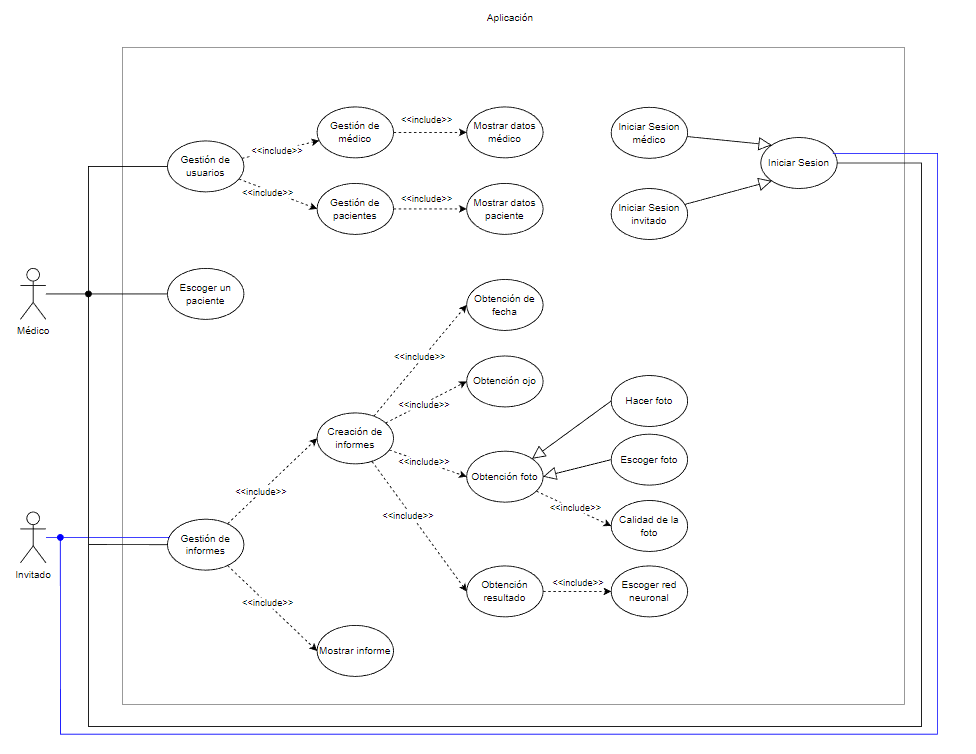
\includegraphics[height=0.8\textheight]{img/Diagrama de casos de uso.png}
         \caption{Diagrama de casos de uso}
         \label{fig:Diagrama de casos de uso}
\end{figure}
\end{landscape}

\textbf{Casos de uso}

\begin{table}[h]
	\centering
	\begin{tabularx}{\linewidth}{ p{0.21\columnwidth} p{0.71\columnwidth} }
		\toprule
		\textbf{CU-1}    & \textbf{Gestión de usuarios}\\
		\toprule
		\textbf{Versión}              & 1.0    \\
		\textbf{Autor}                & Miguel Fuente García \\
		\textbf{Requisitos asociados} & RF-1, RF-1.1, RF-1.1.1, RF-1.2, RF-1.2.1  \\
		\textbf{Descripción}          & Se desea que la aplicación permita gestionar los usuarios. \\
		\textbf{Precondición}         & El médico debe estar identificado, y haya puesto un DNI de paciente valido. \\
		\textbf{Acciones}             &
		\begin{enumerate}
			\def\labelenumi{\arabic{enumi}.}
			\tightlist
			\item El usuario llega a la página principal de la aplicación.
			\item Se ofrece la opción de ver los datos del médico.
                \item Se ofrece la opción de ver los datos del paciente.
		\end{enumerate}\\
		\textbf{Postcondición}        &  \\
		\textbf{Excepciones}          &  \\
		\textbf{Importancia}          & Media  \\
		\bottomrule
	\end{tabularx}
	\caption{CU-1 Gestión de usuarios.}
\end{table}

\begin{table}[h]
	\centering
	\begin{tabularx}{\linewidth}{ p{0.21\columnwidth} p{0.71\columnwidth} }
		\toprule
		\textbf{CU-2}    & \textbf{Gestión de médico}\\
		\toprule
		\textbf{Versión}              & 1.0    \\
		\textbf{Autor}                & Miguel Fuente García \\
		\textbf{Requisitos asociados} & RF-1.1, RF-1.1.1  \\
  
		\textbf{Descripción}          & Se desea que la aplicación permita gestionar los médicos. \\
		\textbf{Precondición}         & El médico debe estar identificado. \\
		\textbf{Acciones}             &
		\begin{enumerate}
			\def\labelenumi{\arabic{enumi}.}
			\tightlist
			\item El usuario selecciona el botón para ver sus datos.
		\end{enumerate}\\
		\textbf{Postcondición}        &  \\
		\textbf{Excepciones}          &  \\
		\textbf{Importancia}          & Baja  \\
		\bottomrule
	\end{tabularx}
	\caption{CU-2 Gestión de médico.}
\end{table}

\begin{table}[p]
	\centering
	\begin{tabularx}{\linewidth}{ p{0.21\columnwidth} p{0.71\columnwidth} }
		\toprule
		\textbf{CU-3}    & \textbf{Mostrar datos médico}\\
		\toprule
		\textbf{Versión}              & 1.0    \\
		\textbf{Autor}                & Miguel Fuente García \\
		\textbf{Requisitos asociados} & RF-1.1.1 \\
		\textbf{Descripción}          & Se desea poder ver los datos de los médicos. \\
		\textbf{Precondición}         & El médico debe estar identificado. \\
		\textbf{Acciones}             &
		\begin{enumerate}
			\def\labelenumi{\arabic{enumi}.}
			\tightlist
			\item La aplicación obtiene los datos del médico de la base de datos.
            \item La aplicación muestra los datos del médico en la interfaz.
		\end{enumerate}\\
		\textbf{Postcondición}        &  \\
		\textbf{Excepciones}          &  \\
		\textbf{Importancia}          & Baja  \\
		\bottomrule
	\end{tabularx}
	\caption{CU-3 Mostrar datos médico.}
\end{table}

\begin{table}[p]
	\centering
	\begin{tabularx}{\linewidth}{ p{0.21\columnwidth} p{0.71\columnwidth} }
		\toprule
		\textbf{CU-4}    & \textbf{Gestión de pacientes}\\
		\toprule
		\textbf{Versión}              & 1.0    \\
		\textbf{Autor}                & Miguel Fuente García \\
		\textbf{Requisitos asociados} & RF-1.2, RF-1.2.1  \\
  
		\textbf{Descripción}          & Se desea que la aplicación permita gestionar los pacientes. \\
		\textbf{Precondición}         & El médico debe estar identificado, y haya puesto un DNI de paciente valido. \\
		\textbf{Acciones}             &
		\begin{enumerate}
			\def\labelenumi{\arabic{enumi}.}
			\tightlist
			\item El usuario selecciona el botón para ver los datos de los pacientes.
		\end{enumerate}\\
		\textbf{Postcondición}        &  \\
		\textbf{Excepciones}          &  \\
		\textbf{Importancia}          & Baja  \\
		\bottomrule
	\end{tabularx}
	\caption{CU-4 Gestión de pacientes.}
\end{table}

\begin{table}[p]
	\centering
	\begin{tabularx}{\linewidth}{ p{0.21\columnwidth} p{0.71\columnwidth} }
		\toprule
		\textbf{CU-5}    & \textbf{Mostrar datos paciente}\\
		\toprule
		\textbf{Versión}              & 1.0    \\
		\textbf{Autor}                & Miguel Fuente García \\
		\textbf{Requisitos asociados} & RF-1.2.1  \\
		\textbf{Descripción}          & Se desea poder ver los datos de los pacientes. \\
		\textbf{Precondición}         & El médico debe estar identificado, y haya puesto un DNI de paciente valido. \\
		\textbf{Acciones}             &
		\begin{enumerate}
			\def\labelenumi{\arabic{enumi}.}
			\tightlist
			\item La aplicación obtiene los datos del paciente de la base de datos.
            \item La aplicación muestra los datos del paciente en la interfaz.
		\end{enumerate}\\
		\textbf{Postcondición}        &  \\
		\textbf{Excepciones}          &  \\
		\textbf{Importancia}          & Baja  \\
		\bottomrule
	\end{tabularx}
	\caption{CU-5 Mostrar datos pacientes.}
\end{table}

\begin{table}[p]
	\centering
	\begin{tabularx}{\linewidth}{ p{0.21\columnwidth} p{0.71\columnwidth} }
		\toprule
		\textbf{CU-6}    & \textbf{Escoger un paciente}\\
		\toprule
		\textbf{Versión}              & 1.0    \\
		\textbf{Autor}                & Miguel Fuente García \\
		\textbf{Requisitos asociados} & RF-4  \\
		\textbf{Descripción}          & Se desea que el médico identificado introduzca el DNI de un paciente para gestionar sus informes o datos. \\
		\textbf{Precondición}         & El médico debe estar identificado. \\
		\textbf{Acciones}             &
		\begin{enumerate}
			\def\labelenumi{\arabic{enumi}.}
			\tightlist
			\item El médico introduce un DNI.
            \item El médico pulsa el botón de comprobación de DNI.
            \item La aplicación comprueba que se haya introducido un número de 8 dígitos.
            \item \begin{enumerate}
                \def\labelenumi{\arabic{enumi}.}
    			\tightlist
                \item Si se ha introducido correctamente, la aplicación sigue con su ejecución.
                \item Si no, se vuelve al paso 1, mostrando un mensaje al usuario de que introduzca un DNI sin la letra final.
            \end{enumerate}
            \item La aplicación comprueba en la base de datos si hay un usuario con ese DNI.
            \item \begin{enumerate}
                \def\labelenumi{\arabic{enumi}.}
    			\tightlist
                \item Si existe, la aplicación muestra el nombre del usuario del DNI.
                \item Si no existe, la aplicación muestra un mensaje de que no existe paciente con ese DNI.
            \end{enumerate}
		\end{enumerate}\\
		\textbf{Postcondición}        & Permite al usuario pasar a la siguiente actividad. \\
		\textbf{Excepciones}          &  \\
		\textbf{Importancia}          & Alta  \\
		\bottomrule
	\end{tabularx}
	\caption{CU-6 Escoger un paciente.}
\end{table}


\begin{table}[p]
	\centering
	\begin{tabularx}{\linewidth}{ p{0.21\columnwidth} p{0.71\columnwidth} }
		\toprule
		\textbf{CU-7}    & \textbf{Gestión de informes}\\
		\toprule
		\textbf{Versión}              & 1.0    \\
		\textbf{Autor}                & Miguel Fuente García \\
		\textbf{Requisitos asociados} & RF-2, RF-2.1, RF-2.1.1, RF-2.1.2, RF-2.1.3, RF-2.1.3.1, RF-2.1.3.2, RF-2.1.3.3, RF-2.1.4, RF-2.1.4.1, RF-2.2  \\
		\textbf{Descripción}          & Se desea que la aplicación permita gestionar los informes. \\
		\textbf{Precondición}         &  \\
		\textbf{Acciones}             &
		\begin{enumerate}
			\def\labelenumi{\arabic{enumi}.}
			\tightlist
			\item Se ofrece la opción de crear informes.
            \item Se ofrece la opción de ver los informes.
            
		\end{enumerate}\\
		\textbf{Postcondición}        &  \\
		\textbf{Excepciones}          &  \\
		\textbf{Importancia}          & Alta  \\
		\bottomrule
	\end{tabularx}
	\caption{CU-7 Gestión de informes.}
\end{table}


\begin{table}[p]
	\centering
	\begin{tabularx}{\linewidth}{ p{0.21\columnwidth} p{0.71\columnwidth} }
		\toprule
		\textbf{CU-8}    & \textbf{Creación de informes}\\
		\toprule
		\textbf{Versión}              & 1.0    \\
		\textbf{Autor}                & Miguel Fuente García \\
		\textbf{Requisitos asociados} & RF-2.1, RF-2.1.1, RF-2.1.2, RF-2.1.3, RF-2.1.3.1, RF-2.1.3.2, RF-2.1.3.3, RF-2.1.4, RF-2.1.4.1  \\
		\textbf{Descripción}          & Se desea que la aplicación permita crear nuevos informes. \\
		\textbf{Precondición}         & Se sabe el paciente en el que añadir el informe. \\
		\textbf{Acciones}             &
		\begin{enumerate}
			\def\labelenumi{\arabic{enumi}.}
			\tightlist
			\item La aplicación obtiene la fecha en la que se crea el informe.
            \item La aplicación obtiene el ojo sobre el que se realiza el informe.
            \item La aplicación obtiene la foto que se guardará en el informe.
            \item La aplicación calcula el resultado del informe
            
		\end{enumerate}\\
		\textbf{Postcondición}        & Se crea un nuevo informe para el paciente y se almacena en la base de datos. \\
		\textbf{Excepciones}          &  \\
		\textbf{Importancia}          & Alta  \\
		\bottomrule
	\end{tabularx}
	\caption{CU-8 Creación de informes.}
\end{table}


\begin{table}[p]
	\centering
	\begin{tabularx}{\linewidth}{ p{0.21\columnwidth} p{0.71\columnwidth} }
		\toprule
		\textbf{CU-9}    & \textbf{Obtención de fecha}\\
		\toprule
		\textbf{Versión}              & 1.0    \\
		\textbf{Autor}                & Miguel Fuente García \\
		\textbf{Requisitos asociados} & RF-2.1.1 \\
		\textbf{Descripción}          & La aplicación debe tomar la fecha en la que se crea el informe. \\
		\textbf{Precondición}         & Se tienen los demás datos para crear el informe. \\
		\textbf{Acciones}             &
		\begin{enumerate}
			\def\labelenumi{\arabic{enumi}.}
			\tightlist
			\item La aplicación obtiene la fecha en la que se crea el informe. 
		\end{enumerate}\\
		\textbf{Postcondición}        & Se crea un nuevo informe para el paciente. \\
		\textbf{Excepciones}          &  \\
		\textbf{Importancia}          & Baja  \\
		\bottomrule
	\end{tabularx}
	\caption{CU-9 Obtención de fecha.}
\end{table}

\begin{table}[p]
	\centering
	\begin{tabularx}{\linewidth}{ p{0.21\columnwidth} p{0.71\columnwidth} }
		\toprule
		\textbf{CU-10}    & \textbf{Obtención de ojo}\\
		\toprule
		\textbf{Versión}              & 1.0    \\
		\textbf{Autor}                & Miguel Fuente García \\
		\textbf{Requisitos asociados} & RF-2.1.2 \\
		\textbf{Descripción}          & La aplicación debe tomar el ojo del informe. \\
		\textbf{Precondición}         & Se sabe el paciente en el que añadir el informe. \\
		\textbf{Acciones}             &
		\begin{enumerate}
			\def\labelenumi{\arabic{enumi}.}
			\tightlist
			\item La aplicación muestra una imagen de ojo derecho y ojo izquierdo.
            \item El usuario escoge sobre cual se realiza el informe.
		\end{enumerate}\\
		\textbf{Postcondición}        & \\
		\textbf{Excepciones}          &  \\
		\textbf{Importancia}          & Baja  \\
		\bottomrule
	\end{tabularx}
	\caption{CU-10 Obtención de ojo.}
\end{table}


\begin{table}[p]
	\centering
	\begin{tabularx}{\linewidth}{ p{0.21\columnwidth} p{0.71\columnwidth} }
		\toprule
		\textbf{CU-11}    & \textbf{Obtención de foto}\\
		\toprule
		\textbf{Versión}              & 1.0    \\
		\textbf{Autor}                & Miguel Fuente García \\
		\textbf{Requisitos asociados} & RF-2.1.3, RF-2.1.3.1, RF-2.1.3.2, RF-2.1.3.3 \\
		\textbf{Descripción}          & La aplicación debe mostrar la opción de como realizar la foto. \\
		\textbf{Precondición}         & Se sabe el paciente en el que añadir el informe y el ojo. \\
		\textbf{Acciones}             &
		\begin{enumerate}
			\def\labelenumi{\arabic{enumi}.}
			\tightlist
			\item La aplicación ofrece un botón para realizar una foto.
            \item La aplicación ofrece un botón para escoger una foto de la galería.
            \item El usuario pulsa una de las opciones, seleccionando una foto.
            \item La aplicación muestra al usuario la imagen obtenida.
            \item La aplicación comprueba la calidad de la imagen.
            \item El usuario puede volver al paso 3, o pasar a la siguiente pantalla.
		\end{enumerate}\\
		\textbf{Postcondición}        & Se ha guardado la foto del informe. \\
		\textbf{Excepciones}          &  \\
		\textbf{Importancia}          & Alta  \\
		\bottomrule
	\end{tabularx}
	\caption{CU-11 Obtención de foto.}
\end{table}

\begin{table}[p]
	\centering
	\begin{tabularx}{\linewidth}{ p{0.21\columnwidth} p{0.71\columnwidth} }
		\toprule
		\textbf{CU-12}    & \textbf{Hacer foto}\\
		\toprule
		\textbf{Versión}              & 1.0    \\
		\textbf{Autor}                & Miguel Fuente García \\
		\textbf{Requisitos asociados} & RF-2.1.3.1 \\
		\textbf{Descripción}          & Se desea que la aplicación permita tomar fotos de la cámara del usuario. \\
		\textbf{Precondición}         & Se sabe el paciente en el que añadir el informe y el ojo. \\
		\textbf{Acciones}             &
		\begin{enumerate}
			\def\labelenumi{\arabic{enumi}.}
			\tightlist
			\item El usuario pulsa el botón de hacer foto.
            \item La aplicación abre la cámara del dispositivo.
            \item El usuario realiza la foto.
            \item La aplicación guarda la imagen.
		\end{enumerate}\\
		\textbf{Postcondición}        & Se ha guardado la foto internamente. \\
		\textbf{Excepciones}          &  \\
		\textbf{Importancia}          & Alta  \\
		\bottomrule
	\end{tabularx}
	\caption{CU-12 Hacer foto.}
\end{table}

\begin{table}[p]
	\centering
	\begin{tabularx}{\linewidth}{ p{0.21\columnwidth} p{0.71\columnwidth} }
		\toprule
		\textbf{CU-13}    & \textbf{Escoger foto}\\
		\toprule
		\textbf{Versión}              & 1.0    \\
		\textbf{Autor}                & Miguel Fuente García \\
		\textbf{Requisitos asociados} & RF-2.1.3.2 \\
		\textbf{Descripción}          & Se desea que la aplicación permita escoger una foto desde la galería del paciente. \\
		\textbf{Precondición}         & Se sabe el paciente en el que añadir el informe y el ojo. \\
		\textbf{Acciones}             &
		\begin{enumerate}
			\def\labelenumi{\arabic{enumi}.}
			\tightlist
			\item El usuario pulsa el botón de escoger foto.
            \item La aplicación abre la galeria del dispositivo.
            \item El usuario selecciona la foto.
            \item La aplicación guarda la imagen seleccionada.
		\end{enumerate}\\
		\textbf{Postcondición}        & Se ha guardado la foto internamente. \\
		\textbf{Excepciones}          &  \\
		\textbf{Importancia}          & Alta  \\
		\bottomrule
	\end{tabularx}
	\caption{CU-13 Escoger foto.}
\end{table}

\begin{table}[p]
	\centering
	\begin{tabularx}{\linewidth}{ p{0.21\columnwidth} p{0.71\columnwidth} }
		\toprule
		\textbf{CU-14}    & \textbf{Calidad foto}\\
		\toprule
		\textbf{Versión}              & 1.0    \\
		\textbf{Autor}                & Miguel Fuente García \\
		\textbf{Requisitos asociados} & RF-2.1.3.3 \\
		\textbf{Descripción}          & Se desea implementar un sistema que permita comprobar que la foto tomada es
de calidad. \\
		\textbf{Precondición}         & Se sabe el paciente en el que añadir el informe y el ojo. Y se ha mostrado la foto al usuario. \\
		\textbf{Acciones}             &
		\begin{enumerate}
			\def\labelenumi{\arabic{enumi}.}
			\tightlist
			\item La aplicación obtiene la imagen mostrada al usuario.
            \item La aplicación trabaja en segundo plano.
            \item La aplicación realiza un preprocesado a la imagen.
            \item La aplicación introduce a la red neuronal de calidad la imagen.
            \item La aplicación obtiene el resultado.
            \item \begin{enumerate}
                \item Si es una calidad apta, se permite al usuario avanzar a la siguiente actividad.
                \item Si es una calidad no apta, se muestra un mensaje de omitir comprobación de calidad, que si pulsa, permite al usuario avanzar a la siguiente actividad.
            \end{enumerate}
		\end{enumerate}\\
		\textbf{Postcondición}        & Se ha comprobado la calidad de la foto. \\
		\textbf{Excepciones}          &  \\
		\textbf{Importancia}          & Alta  \\
		\bottomrule
	\end{tabularx}
	\caption{CU-14 Calidad foto.}
\end{table}

\begin{table}[p]
	\centering
	\begin{tabularx}{\linewidth}{ p{0.21\columnwidth} p{0.71\columnwidth} }
		\toprule
		\textbf{CU-15}    & \textbf{Obtención del resultado}\\
		\toprule
		\textbf{Versión}              & 1.0    \\
		\textbf{Autor}                & Miguel Fuente García \\
		\textbf{Requisitos asociados} & RF-2.1.4 \\
		\textbf{Descripción}          & Se desea que la aplicación de un resultado basado en una red neuronal. \\
		\textbf{Precondición}         & Se sabe el paciente en el que añadir el informe y el ojo. Y se ha guardado la foto. \\
		\textbf{Acciones}             &
		\begin{enumerate}
			\def\labelenumi{\arabic{enumi}.}
			\tightlist
			\item La aplicación obtiene la imagen mostrada al usuario.
            \item El usuario selecciona las redes neuronales con las que analizar la imagen.
            \item La aplicación obtiene los resultados y calcula la moda y en caso de empate, la media.
		\end{enumerate}\\
		\textbf{Postcondición}        & Se crea el informe con todos los atributos. \\
		\textbf{Excepciones}          &  \\
		\textbf{Importancia}          & Alta  \\
		\bottomrule
	\end{tabularx}
	\caption{CU-15 Obtención del resultado.}
\end{table}

\begin{table}[p]
	\centering
	\begin{tabularx}{\linewidth}{ p{0.21\columnwidth} p{0.71\columnwidth} }
		\toprule
		\textbf{CU-16}    & \textbf{Escoger red neuronal}\\
		\toprule
		\textbf{Versión}              & 1.0    \\
		\textbf{Autor}                & Miguel Fuente García \\
		\textbf{Requisitos asociados} & RF-2.1.4.1 \\
		\textbf{Descripción}          & Se desea que el usuario pueda elegir con que red neuronal analizar la imagen con la que obtener los resultados. \\
		\textbf{Precondición}         & Se tiene la imagen para el informe. \\
		\textbf{Acciones}             &
		\begin{enumerate}
			\def\labelenumi{\arabic{enumi}.}
			\tightlist
			\item El usuario selecciona las redes neuronales con las que analizar la imagen.
            \item La aplicación preprocesa la imagen para las redes neuronales seleccionadas.
            \item La aplicación introduce las imágenes preprocesadas en sus respectivos modelos.
		\end{enumerate}\\
		\textbf{Postcondición}        & La aplicación obtiene los resultados y calcula la moda y en caso de empate, la media. \\
		\textbf{Excepciones}          &  \\
		\textbf{Importancia}          & Alta  \\
		\bottomrule
	\end{tabularx}
	\caption{CU-16 Escoger red neuronal.}
\end{table}

\begin{table}[p]
	\centering
	\begin{tabularx}{\linewidth}{ p{0.21\columnwidth} p{0.71\columnwidth} }
		\toprule
		\textbf{CU-17}    & \textbf{Mostrar informe}\\
		\toprule
		\textbf{Versión}              & 1.0    \\
		\textbf{Autor}                & Miguel Fuente García \\
		\textbf{Requisitos asociados} & RF-2.2 \\
		\textbf{Descripción}          & Se desea poder ver los informes según el paciente. \\
		\textbf{Precondición}         & Se sabe el paciente. \\
		\textbf{Acciones}             &
		\begin{enumerate}
			\def\labelenumi{\arabic{enumi}.}
			\tightlist
			\item El usuario selecciona la opción para ver los informes del paciente.
            \item La aplicación muestra un listado de los informes del paciente ordenados de más nuevos a más viejos.
            \item La aplicación muestra los informes de 3 en 3 permitiendo avanzar y retroceder entre el listado.
		\end{enumerate}\\
		\textbf{Postcondición}        &  \\
		\textbf{Excepciones}          &  \\
		\textbf{Importancia}          & Media  \\
		\bottomrule
	\end{tabularx}
	\caption{CU-17 Mostrar informe.}
\end{table}

\begin{table}[p]
	\centering
	\begin{tabularx}{\linewidth}{ p{0.21\columnwidth} p{0.71\columnwidth} }
		\toprule
		\textbf{CU-18}    & \textbf{Iniciar sesión}\\
		\toprule
		\textbf{Versión}              & 1.0    \\
		\textbf{Autor}                & Miguel Fuente García \\
		\textbf{Requisitos asociados} & RF-3, RF-3.1, RF-3.2 \\
		\textbf{Descripción}          & Se desea que la aplicación permita iniciar sesión. \\
		\textbf{Precondición}         & El usuario debe estar registrado en la base de datos. \\
		\textbf{Acciones}             &
		\begin{enumerate}
			\def\labelenumi{\arabic{enumi}.}
			\tightlist
			\item La aplicación ofrece iniciar sesión por email y contraseña.
            \item La aplicación ofrece iniciar sesión como invitado.

		\end{enumerate}\\
		\textbf{Postcondición}        &  \\
		\textbf{Excepciones}          &  \\
		\textbf{Importancia}          & Media  \\
		\bottomrule
	\end{tabularx}
	\caption{CU-18 Iniciar sesión.}
\end{table}

\begin{table}[p]
	\centering
	\begin{tabularx}{\linewidth}{ p{0.21\columnwidth} p{0.71\columnwidth} }
		\toprule
		\textbf{CU-19}    & \textbf{Iniciar sesión como médico}\\
		\toprule
		\textbf{Versión}              & 1.0    \\
		\textbf{Autor}                & Miguel Fuente García \\
		\textbf{Requisitos asociados} & RF-3.1 \\
		\textbf{Descripción}          & Los médicos pueden iniciar sesión con su email y su contraseña. \\
		\textbf{Precondición}         & El usuario debe estar registrado en la base de datos. \\
		\textbf{Acciones}             &
		\begin{enumerate}
			\def\labelenumi{\arabic{enumi}.}
			\tightlist
			\item El usuario introduce el email y la contraseña.
            \item El usuario pulsa el botón para iniciar sesión.
            \item \begin{enumerate}
                \item La aplicación comprueba si no se han introducido campos vacios.
                \item La aplicación comprueba que el usuario existe.
                \item La aplicación comprueba si la contraseña de ese usuario es la introducida.
            \end{enumerate}
            \item \begin{enumerate}
                \item Si cumple las 3 condiciones anteriores, el usuario inicia sesión.
                \item Si no, se muestra al usuario un mensaje de que el email o contraseña son incorrectos.
            \end{enumerate}
		\end{enumerate}\\
		\textbf{Postcondición}        &  \\
		\textbf{Excepciones}          &  \\
		\textbf{Importancia}          & Media  \\
		\bottomrule
	\end{tabularx}
	\caption{CU-19 Iniciar sesión como médico.}
\end{table}

\begin{table}[p]
	\centering
	\begin{tabularx}{\linewidth}{ p{0.21\columnwidth} p{0.71\columnwidth} }
		\toprule
		\textbf{CU-20}    & \textbf{Iniciar sesión como invitado}\\
		\toprule
		\textbf{Versión}              & 1.0    \\
		\textbf{Autor}                & Miguel Fuente García \\
		\textbf{Requisitos asociados} & RF-3.1 \\
		\textbf{Descripción}          & Los médicos pueden iniciar sesión con su email y su contraseña. \\
		\textbf{Precondición}         & El usuario debe estar registrado en la base de datos. \\
		\textbf{Acciones}             &
		\begin{enumerate}
			\def\labelenumi{\arabic{enumi}.}
			\tightlist
			\item El usuario pulsa el botón para iniciar sesión como invitado.
            \item La aplicación inicia sesión como médico ``invitado'' y paciente ``invitado''.
  
		\end{enumerate}\\
		\textbf{Postcondición}        &  \\
		\textbf{Excepciones}          &  \\
		\textbf{Importancia}          & Media  \\
		\bottomrule
	\end{tabularx}
	\caption{CU-20 Iniciar sesión como invitado.}
\end{table}